% Options for packages loaded elsewhere
\PassOptionsToPackage{unicode}{hyperref}
\PassOptionsToPackage{hyphens}{url}
%
\documentclass[
]{article}
\usepackage{amsmath,amssymb}
\usepackage{iftex}
\ifPDFTeX
  \usepackage[T1]{fontenc}
  \usepackage[utf8]{inputenc}
  \usepackage{textcomp} % provide euro and other symbols
\else % if luatex or xetex
  \usepackage{unicode-math} % this also loads fontspec
  \defaultfontfeatures{Scale=MatchLowercase}
  \defaultfontfeatures[\rmfamily]{Ligatures=TeX,Scale=1}
\fi
\usepackage{lmodern}
\ifPDFTeX\else
  % xetex/luatex font selection
\fi
% Use upquote if available, for straight quotes in verbatim environments
\IfFileExists{upquote.sty}{\usepackage{upquote}}{}
\IfFileExists{microtype.sty}{% use microtype if available
  \usepackage[]{microtype}
  \UseMicrotypeSet[protrusion]{basicmath} % disable protrusion for tt fonts
}{}
\makeatletter
\@ifundefined{KOMAClassName}{% if non-KOMA class
  \IfFileExists{parskip.sty}{%
    \usepackage{parskip}
  }{% else
    \setlength{\parindent}{0pt}
    \setlength{\parskip}{6pt plus 2pt minus 1pt}}
}{% if KOMA class
  \KOMAoptions{parskip=half}}
\makeatother
\usepackage{xcolor}
\usepackage[margin=1in]{geometry}
\usepackage{longtable,booktabs,array}
\usepackage{calc} % for calculating minipage widths
% Correct order of tables after \paragraph or \subparagraph
\usepackage{etoolbox}
\makeatletter
\patchcmd\longtable{\par}{\if@noskipsec\mbox{}\fi\par}{}{}
\makeatother
% Allow footnotes in longtable head/foot
\IfFileExists{footnotehyper.sty}{\usepackage{footnotehyper}}{\usepackage{footnote}}
\makesavenoteenv{longtable}
\usepackage{graphicx}
\makeatletter
\def\maxwidth{\ifdim\Gin@nat@width>\linewidth\linewidth\else\Gin@nat@width\fi}
\def\maxheight{\ifdim\Gin@nat@height>\textheight\textheight\else\Gin@nat@height\fi}
\makeatother
% Scale images if necessary, so that they will not overflow the page
% margins by default, and it is still possible to overwrite the defaults
% using explicit options in \includegraphics[width, height, ...]{}
\setkeys{Gin}{width=\maxwidth,height=\maxheight,keepaspectratio}
% Set default figure placement to htbp
\makeatletter
\def\fps@figure{htbp}
\makeatother
\setlength{\emergencystretch}{3em} % prevent overfull lines
\providecommand{\tightlist}{%
  \setlength{\itemsep}{0pt}\setlength{\parskip}{0pt}}
\setcounter{secnumdepth}{-\maxdimen} % remove section numbering
\ifLuaTeX
  \usepackage{selnolig}  % disable illegal ligatures
\fi
\IfFileExists{bookmark.sty}{\usepackage{bookmark}}{\usepackage{hyperref}}
\IfFileExists{xurl.sty}{\usepackage{xurl}}{} % add URL line breaks if available
\urlstyle{same}
\hypersetup{
  pdftitle={Analyzing Insurance Claims for Future Financial Safeguard},
  hidelinks,
  pdfcreator={LaTeX via pandoc}}

\title{Analyzing Insurance Claims for Future Financial Safeguard}
\author{}
\date{\vspace{-2.5em}2023-12-17}

\begin{document}
\maketitle

\hypertarget{abstract}{%
\subsection{Abstract}\label{abstract}}

In the realm of insurance, the anticipation of claims plays a pivotal
role in risk management and financial planning. This project delves into
the challenge of predicting insurance claims, a task made intricate by a
dataset characterized by its modest sample size and a slight imbalance
between claimed and unclaimed instances. The objective is to surmount
these obstacles and construct a robust predictive model capable of
accurately classifying insurance claims. The project will navigate
through methodologies to address imbalances, optimize feature
extraction, and employ advanced predictive modeling techniques such as
classification and regression trees, random forest, xgboost algorithms,
statistical models such as logit and probit, and Support Vector Machines
(SVM).

The SVM model, known for its effectiveness in both classification and
regression tasks, will be explored to enhance the predictive
capabilities of the model. By leveraging SVM's ability to find optimal
decision boundaries, we aim to further refine our predictive model. This
comprehensive approach, encompassing a variety of advanced modeling
techniques, seeks to contribute valuable insights to the field of
insurance analytics, enabling more informed decision-making and risk
assessment.

\newpage

\hypertarget{introduction}{%
\subsection{Introduction}\label{introduction}}

Within the scope of insurance analytics, the task of predicting
insurance claims has emerged as a significant focal point, garnering
increased attention in recent years. This heightened interest is
attributed to the critical role that accurate predictions play in
effective risk management and strategic financial planning within the
insurance industry. Numerous research endeavors have been dedicated to
the development of robust predictive models, each tailored to address
the unique challenges posed by insurance datasets.

The complexity of this endeavor is compounded by the inherent
characteristics of the dataset at hand. With a relatively modest sample
size, the dataset presents challenges in capturing the diverse scenarios
that may lead to insurance claims. Additionally, there is a slight
imbalance between instances where claims are made and those where claims
are not, adding an extra layer of complexity to the predictive modeling
task.

Addressing these challenges requires sophisticated methodologies that
can effectively navigate the nuances of the data. Researchers have
explored various strategies to optimize predictive model performance,
considering factors such as imbalances in the dataset and the need for
accurate classification. As we delve into this project, the goal is to
overcome these obstacles and construct a predictive model that not only
captures the intricacies of the data but also generalizes well to new,
unseen instances. The methodologies employed will span techniques for
handling imbalanced data, optimizing feature extraction, and leveraging
advanced modeling algorithms, including classification and regression
trees, random forest, xgboost, support vector machines and statistical
models such as logistic regression and probit regression.

By addressing the challenges head-on and employing state-of-the-art
methodologies, the project aims to contribute valuable insights to the
evolving landscape of insurance analytics. The overarching objective is
to empower decision-makers in the insurance industry with accurate and
actionable predictions, facilitating more informed choices in risk
assessment and financial planning.

\newpage

\hypertarget{literature-review}{%
\subsection{Literature Review}\label{literature-review}}

Class Imbalance and Sample Size Concerns:

The inherent challenges associated with modest sample sizes and class
imbalances in insurance datasets have been widely acknowledged.
Researchers have explored various strategies to mitigate these issues,
including oversampling techniques, undersampling approaches, and the
synthesis of artificial instances to balance the distribution of claimed
and unclaimed instances. Notable studies, have demonstrated the efficacy
of these methods in enhancing the predictive performance of models in
similar contexts.

Feature Extraction and Optimization:

Feature extraction plays a pivotal role in the predictive accuracy of
models. Researchers have delved into optimizing feature selection
techniques to identify the most informative variables. Dimensionality
reduction methods, such as Variable Selection method with forward
elimination, backward elimination, both and Variable importance
parameter have been explored to enhance model interpretability and
generalization performance.

Predictive Modeling Techniques:

The literature is rich with studies employing various predictive
modeling techniques for insurance claim prediction. Classification and
regression trees (CART), renowned for their interpretability and
flexibility, have been extensively utilized. Additionally, ensemble
methods such as random forest and xgboost algorithms have gained
popularity for their ability to handle complex interactions and improve
predictive accuracy. These techniques have been benchmarked against
traditional statistical models, including logistic (logit) and probit
regression, revealing nuanced insights into the trade-offs between
interpretability and predictive power.

Contributions to Insurance Analytics:

By addressing the intricacies of insurance datasets, these studies
collectively contribute to the advancement of insurance analytics.
Insights gained from predictive models enable stakeholders to make more
informed decisions, refine risk assessment strategies, and ultimately
bolster the financial stability of insurance providers. The literature
underscores the necessity of a multi-faceted approach that integrates
advanced statistical learning methodologies to harness the full
predictive potential of insurance data.

In summary, the existing body of literature provides a comprehensive
foundation for the current project's objectives. By building upon these
insights and addressing specific challenges posed by the dataset at
hand, this study aspires to add valuable contributions to the ongoing
discourse in insurance claim prediction.

\newpage

\hypertarget{data-description}{%
\subsection{Data Description}\label{data-description}}

This data frame contains the following columns:

\begin{itemize}
\tightlist
\item
  \textbf{age}: Age of the policyholder.
\item
  \textbf{sex}: Gender of the policyholder (female=0, male=1).
\item
  \textbf{bmi}: Body mass index, providing an understanding of body
  weight relative to height (kg / m \^{} 2).
\item
  \textbf{steps}: Average walking steps per day of the policyholder.
\item
  \textbf{children}: Number of children/dependents of the policyholder.
\item
  \textbf{smoker}: Smoking status of the policyholder (non-smoke=0;
  smoker=1).
\item
  \textbf{region}: The residential area of the policyholder in the US
  (northeast=0, northwest=1, southeast=2, southwest=3).
\item
  \textbf{charges}: Individual medical costs billed by health insurance.
\item
  \textbf{insuranceclaim}: Insurance claim status (yes=1, no=0).
\end{itemize}

The dataset comprises 1338 observations, encompassing explanatory
variables such as age, sex, BMI, children, smoker, region, and charges,
along with response variables like insurance claim.

Categorical predictor variables, including sex, children, smoker, and
region, contain intermediate levels (2, 6, 2, 4, respectively). The
dataset consists of 662 females and 675 males. Non-smokers total 1063,
while smokers amount to 274. Four regions are represented, with mappings
northeast=0, northwest=1, southeast=2, southwest=3, and counts of 324,
324, 364, and 325, respectively. The ``children'' feature indicates the
number of dependents: 573 with no dependents, 324 with 1 dependent, 240
with 2 dependents, 157 with 3 dependents, 25 with 4 dependents, and 18
with 5 dependents.

The response variables exhibit two levels, 0 and 1, denoting no claim
and claim, respectively, with counts of 555 and 782.

Dirstribution of the Response variable

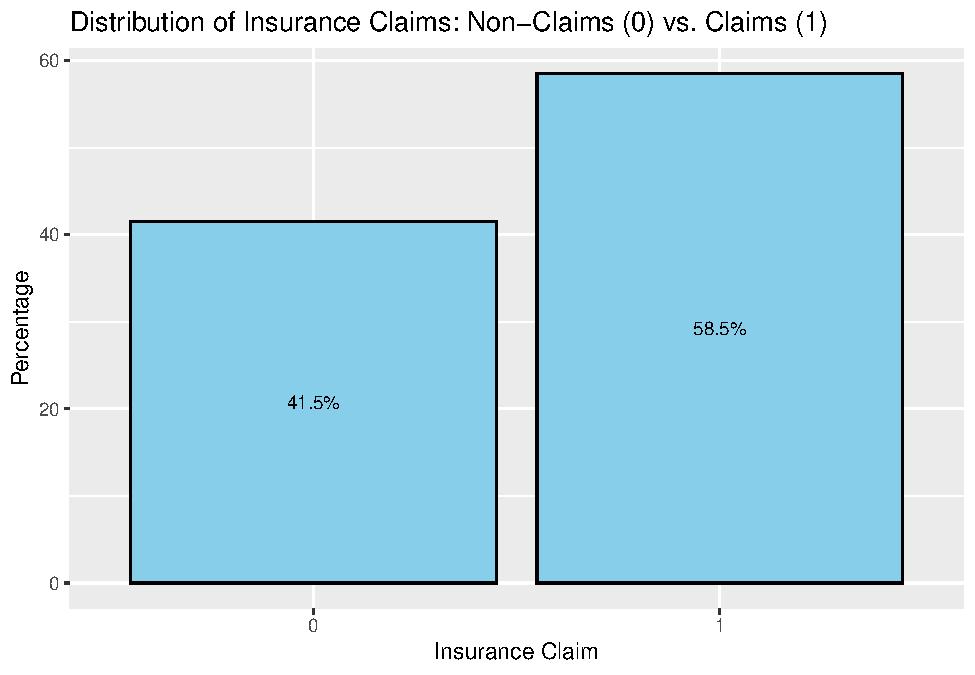
\includegraphics{Insurance_Claim_Prediction_Report_files/figure-latex/unnamed-chunk-2-1.pdf}

\newpage

\hypertarget{goal}{%
\subsection{Goal}\label{goal}}

In the domain of insurance, where uncertainty meets financial planning,
our mission is crystal clear: predict the unpredictable. The heart of
this project beats with the ambition to not just foresee insurance
claims but to unravel the variables that wield the most influence in
shaping these predictions.

\hypertarget{statistical-methods}{%
\subsection{Statistical Methods}\label{statistical-methods}}

\begin{enumerate}
\def\labelenumi{\arabic{enumi}.}
\tightlist
\item
  \textbf{Logistic Regression (Logit):} Statistical model for binary
  classification.
\end{enumerate}

Basis on the response variable with 0's and 1's which is a binomial we
can apply binary logit model

A \textbf{binary random variable} \(Y\) can assume only one of two
possible values, a value of \(1\) (Yes) or a value of \(0\) (No). and
probability mass function (p.m.f.)

\[
p(y; \pi) = \pi^y (1-\pi)^{1-y},~y = 0 \mbox{ or } 1; 0 \le \pi  \le 1. 
\] \{\#eq-pmfBern\}

A useful transformation of \(\pi\) is the logit (or, log-odds)
transformation:

\[
\text{logit}(\pi) = \log \left(\frac{\pi}{1-\pi}\right)
\] \{\#eq-logitpi\}

Let \(\eta = \text{logit}(\pi)\). After some algebra, we see that we can
uniquely write \(\pi\) as a function of \(\eta\), i.e., the inverse
transformation is

\[
\pi = \frac{\exp(\eta)}{1+\exp(\eta)}
\] \{\#eq-invlogit\}

\begin{enumerate}
\def\labelenumi{\arabic{enumi}.}
\tightlist
\item
  Full Binary logit model was fitted on the data where the response
  variable is insuranceclaims and the remaining variables such as sex,
  children, bmi, smokers, age, region and charges.
\end{enumerate}

Following are the null and alternative hypothesis.

\textbf{Null Hypothesis (\(H_0\)):} \[ H_0: \beta_j = 0 \]

The null hypothesis asserts that there is no association between the
independent variable \(X_j\) and the log-odds of the dependent variable
being in the ``success'' category.

\textbf{Alternative Hypothesis (\(H_1\)):} \[ H_1: \beta_j \neq 0 \]

The alternative hypothesis suggests that the independent variable
\(X_j\) does have a significant association with the log-odds of the
event.

After fitting the full and both Logit Model we reject the null
hypothesis with extremely less p-value,

\textbf{Age, BMI, number of children, and smoking} status appear to be
significant predictors of insurance claims. - Charges and region may not
be statistically significant predictors in this model.

\begin{verbatim}
##  933 1117 
##  759  894
\end{verbatim}

\begin{verbatim}
##  933 1117 
##  759  894
\end{verbatim}

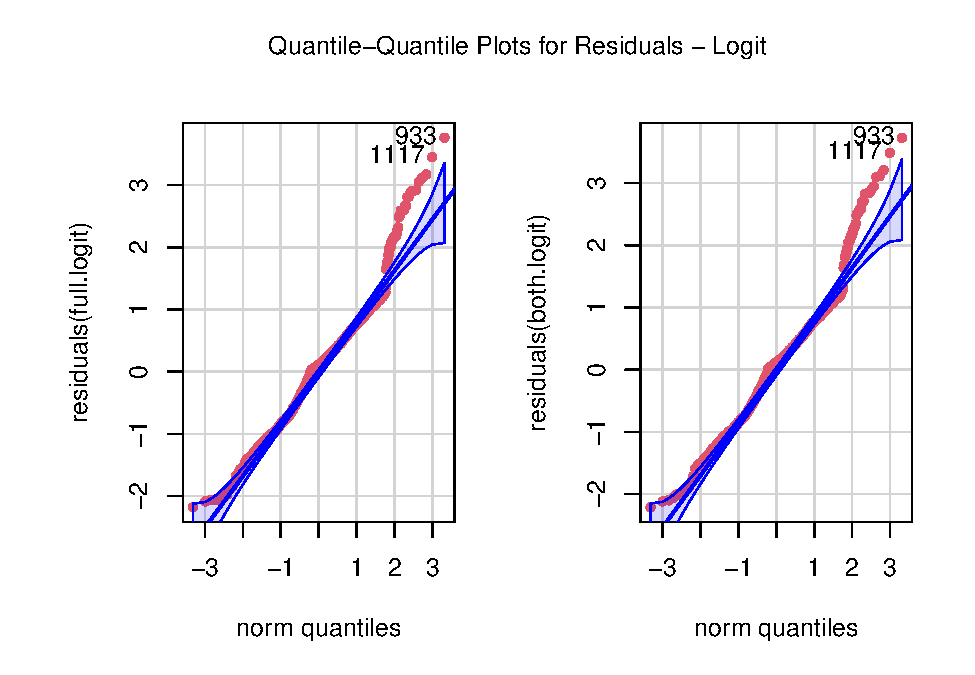
\includegraphics{Insurance_Claim_Prediction_Report_files/figure-latex/unnamed-chunk-3-1.pdf}
From the above residual plot we can observe most of the data points were
normal except few data points. Fitted the model by removing the outliers
with the standard deviation greater than 3 times however even though the
AIC values got down \textbf{normality assumption did not satisfy}.

\begin{enumerate}
\def\labelenumi{\arabic{enumi}.}
\setcounter{enumi}{1}
\tightlist
\item
  \textbf{Probit Regression (Probit):} Alternative statistical model.
\end{enumerate}

Starting with the standard normal c.d.f \(\phi(z)\) which lies in the
interval \([0, 1]\), the probit (or inverse normal c.d.f.) link assumes
that

\[
\phi^{-1}(\pi_i) = \eta_i 
\] \{\#eq-probit1\}

so that

\[
\pi_i = \Phi(\eta_i)
\] \{\#eq-probit2\}

where \(\eta_i\) is given by @eq-binarysys as

\[
\eta_i =  \beta_0 + \sum_{j=1}^p  \beta_j X_{i,j} = \mathbf{x}_i' \boldsymbol{\beta}.
\]

\textbf{Null Hypothesis (\(H_0\)):} \[ H_0: \beta_j = 0 \]

The null hypothesis asserts that there is no association between the
independent variable \(X_j\) and the probability of the dependent
variable being in the ``success'' category.

\textbf{Alternative Hypothesis (\(H_1\)):} \[ H_1: \beta_j \neq 0 \]

After fitting the probit model, we reject the null hypothesis as there
is a significant asscociation for some variable to the response
variable.

The logistic regression model was fitted to predict insurance claims
based on various factors. The significant predictors include age, BMI,
number of children, smoking status, and certain regions. Age and BMI
showed positive associations with the likelihood of making an insurance
claim, while having children had a negative impact, with the odds
decreasing as the number of children increased. Smoking status was a
strong positive predictor, indicating higher odds for smokers. The
specific impact of regions varied, with some regions contributing to a
decrease in the odds of a claim. The model's overall significance was
confirmed by the Wald test (Chi-square = 418.14, df = 13, p \textless{}
2e-16). The model's goodness of fit was assessed using the Deviance
statistic, with a residual deviance of 765.01 on 1055 degrees of
freedom. The AIC value was 793.01, indicating a relatively good fit.
Overall, the logistic regression model provides insights into the
factors influencing insurance claims, with age, BMI, smoking status, and
region being key determinants.

\begin{verbatim}
##  933 1117 
##  759  894
\end{verbatim}

\begin{verbatim}
##  933 1117 
##  759  894
\end{verbatim}

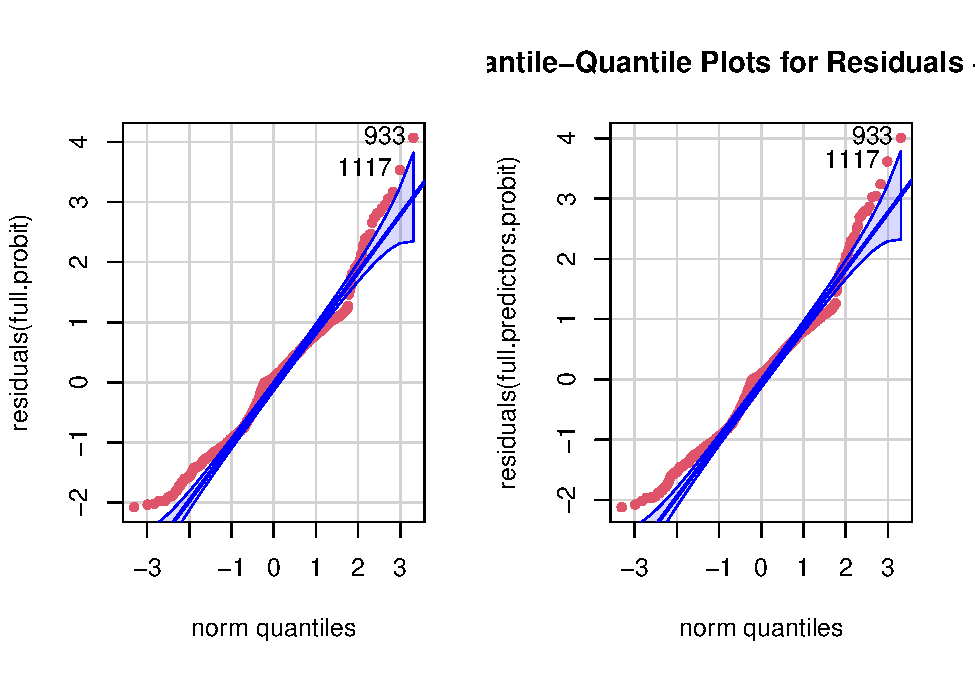
\includegraphics{Insurance_Claim_Prediction_Report_files/figure-latex/unnamed-chunk-4-1.pdf}
From the above residual plot it is clear that most of the data points
were normal except few data points. Fitted the model by removing the
outliers with the standard deviation greater than 3 times however even
though the AIC values got down \textbf{normality assumption did not
satisfy}.

\begin{enumerate}
\def\labelenumi{\arabic{enumi}.}
\setcounter{enumi}{2}
\tightlist
\item
  \textbf{Classification and Regression Trees (CART):} Decision tree
  models for classification.
\end{enumerate}

We define two impurity measures, Gini index and entropy, for classifying
a response with \(J\) categories. The \textbf{Gini index} is defined by
\[
\mbox{Gini index} = 1 - \sum_{j=1}^J p^2_j,  
\] \{\#eq-gini-index\}

where \(p_j = P(Y \in \mbox{class} j),~j=1,\ldots,J\). Gini index lies
in \([0, 1]\). The value \(0\) denotes a pure classification where all
the cases belong to a single class, while \(1\) indicates a random
distribution of cases across the \(J\) classes. A Gini index of \(0.5\)
shows an equal distribution of cases over some classes.

\[
\text{Cost}_{CP}(\mbox{Tree}) = \mbox{Error(Tree)} + Cp  \ \mathcal{N}(\mbox{Tree}),
\] where, Error(Tree) is the fraction of misclassified cases and
\(\mathcal{N}(\mbox{Tree})\) is the number of leaf nodes in the tree.

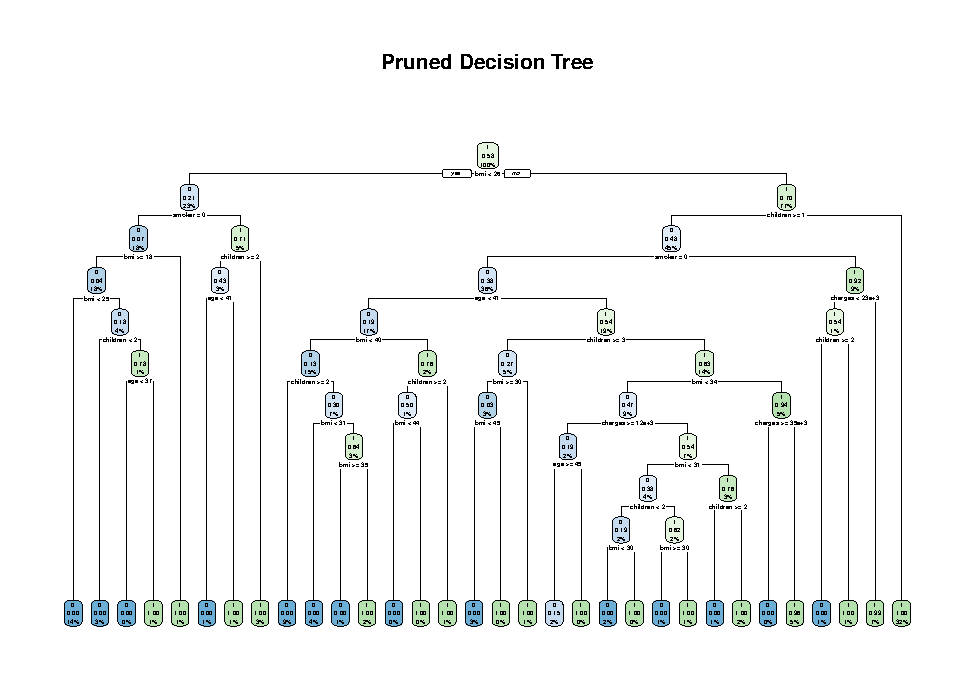
\includegraphics{Insurance_Claim_Prediction_Report_files/figure-latex/unnamed-chunk-5-1.pdf}
Fitting the CART algorithm and pruning the tree we can view the refined
tree with all the conditions at each level including the details of root
node error and percent of variability. At the low level of the tree we
can view the leaf nodes which classies the response vairables based on
the above conditions. Also, implemented tree by various cp values such
as 0.0001 and 0.1 which yielded the similar result.

\begin{enumerate}
\def\labelenumi{\arabic{enumi}.}
\setcounter{enumi}{3}
\tightlist
\item
  \textbf{Random Forest:} Ensemble model for enhanced accuracy.
\end{enumerate}

The random forest (RF) is an ensemble learning method which consists of
aggregating a large number of decision trees to avoid overfitting and
build a better classification model

The Ranger regression model, built on the insurance data, comprises 500
trees with a sample size of 1070 and incorporates seven independent
variables. For each split, the model randomly samples three variables,
and the target node size is set at 5. The variable importance is
assessed based on impurity, and the split rule is determined by
variance. The out-of-bag prediction error (mean squared error) is
measured at 0.03085552, indicating a relatively low prediction error,
while the R-squared value stands at 0.8730195, signifying a high
proportion of explained variance in the target variable. These results
collectively suggest that the Ranger regression model performs well in
predicting insurance claims, offering accuracy and a strong ability to
capture variability in the data.

\begin{verbatim}
## # A tibble: 7 x 2
##   Variable Importance
##   <chr>         <dbl>
## 1 bmi           97.6 
## 2 children      72.9 
## 3 charges       33.1 
## 4 smoker        23.0 
## 5 age           21.0 
## 6 region         3.55
## 7 sex            1.33
\end{verbatim}

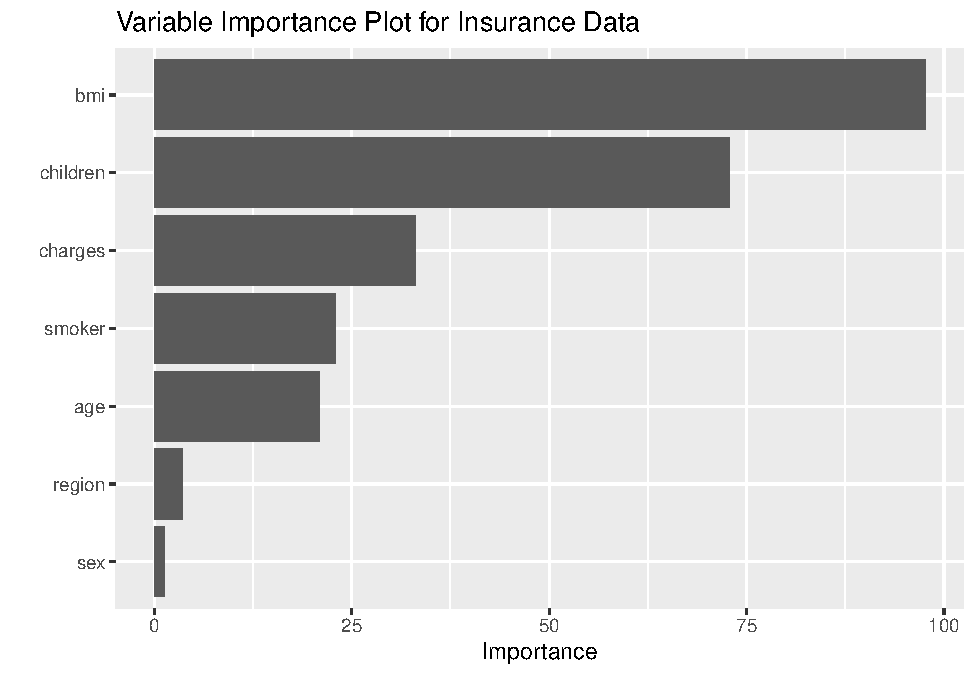
\includegraphics{Insurance_Claim_Prediction_Report_files/figure-latex/unnamed-chunk-6-1.pdf}
Bmi, Children, charges, smoker are having more values from the above
\textbf{Variable Importance Plot} which indicates the impact those
variables shows on predicting the response variable. Implemented the
random forest by dropping the columns age, region and sex one after the
other and observed improvement in the accuracy on both the train and
test data. A popular variant is the gradient boosting algorithm, and
XGBoost (acronym for eXtreme Gradient Boosting.

\begin{enumerate}
\def\labelenumi{\arabic{enumi}.}
\setcounter{enumi}{4}
\tightlist
\item
  \textbf{XGBoost Algorithm:} Efficient algorithm for structured data.
\end{enumerate}

For binary response modeling, the idea of boosting was introduced to
improve the performance of weak learners. This was done by resampling
the training data responses, giving more weight to the misclassified
ones, thereby leading to a refined classifier (binary model) which would
boost feature performance, especially in ambiguous areas of the feature
space.

Plot for the xgboost tree was specified in the following file
\textbf{tree\_plot.html}.

From the above plot we can interpret that the a condition was applied on
the chargers column as it's gain value is more with 74 where if it is
less than 30175.7773 then it check for the children(gain is 73 ) else
bmi(2.4) and later we have further splits based on this.

By increasing the rounds from 2 to 15 there is an increase in the
accuracy on both the train and test dataset.

\begin{enumerate}
\def\labelenumi{\arabic{enumi}.}
\setcounter{enumi}{5}
\tightlist
\item
  \textbf{Support Vector Machines}
\end{enumerate}

\textbf{Hyperplane}: The decision boundary that separates the data into
classes. For a two-dimensional space, the hyperplane is a line; for
three dimensions, it's a plane, and so on.

\textbf{Margin}: The margin is the distance between the hyperplane and
the nearest data point from either class. SVM seeks to maximize this
margin, as a larger margin often leads to better generalization to
unseen data.

\textbf{Support Vectors}: Support vectors are the data points that are
closest to the hyperplane and have a significant influence on its
position. These points play a crucial role in determining the optimal
hyperplane.

\textbf{Kernel Trick}: SVM can handle non-linear relationships in the
data by transforming the features into a higher-dimensional space. This
is achieved using a kernel function, which computes the dot product in
this higher-dimensional space without explicitly calculating the
transformed features.

\textbf{Regularization Parameter (C)}: It controls the trade-off between
having a smooth decision boundary and correctly classifying the training
data. A smaller C value allows for a larger margin but may misclassify
some training points, while a larger C value aims to classify all
training points correctly but may result in a smaller margin.

The Support Vector Machine (SVM) model is configured as an
epsilon-regression with a linear kernel for predicting insurance claims.
With 981 identified support vectors, the model demonstrates a nuanced
understanding of critical data points. Evaluation on the test set yields
an accuracy of approximately 86.64\%, with a sensitivity of 83.33\% and
specificity of 88.98\%. These metrics showcase the model's effectiveness
in correctly predicting both positive (claims) and negative instances.
The SVM decision boundary, visualized through a plot, illustrates the
model's ability to discriminate between insurance claim categories in
the training set. Overall, the SVM model exhibits robust performance in
predicting insurance claims, crucial for risk assessment in the realm of
insurance analytics.

\hypertarget{results-from-the-analyses}{%
\subsection{Results from the Analyses}\label{results-from-the-analyses}}

\begin{longtable}[]{@{}
  >{\raggedright\arraybackslash}p{(\columnwidth - 12\tabcolsep) * \real{0.3511}}
  >{\raggedleft\arraybackslash}p{(\columnwidth - 12\tabcolsep) * \real{0.0957}}
  >{\raggedleft\arraybackslash}p{(\columnwidth - 12\tabcolsep) * \real{0.1064}}
  >{\raggedleft\arraybackslash}p{(\columnwidth - 12\tabcolsep) * \real{0.1064}}
  >{\raggedleft\arraybackslash}p{(\columnwidth - 12\tabcolsep) * \real{0.1064}}
  >{\raggedleft\arraybackslash}p{(\columnwidth - 12\tabcolsep) * \real{0.1170}}
  >{\raggedleft\arraybackslash}p{(\columnwidth - 12\tabcolsep) * \real{0.1170}}@{}}
\caption{Decision Trees - Model Performance Results}\tabularnewline
\toprule\noalign{}
\begin{minipage}[b]{\linewidth}\raggedright
Model
\end{minipage} & \begin{minipage}[b]{\linewidth}\raggedleft
Test\_Acc
\end{minipage} & \begin{minipage}[b]{\linewidth}\raggedleft
Test\_sens
\end{minipage} & \begin{minipage}[b]{\linewidth}\raggedleft
Test\_spec
\end{minipage} & \begin{minipage}[b]{\linewidth}\raggedleft
Train\_Acc
\end{minipage} & \begin{minipage}[b]{\linewidth}\raggedleft
Train\_sens
\end{minipage} & \begin{minipage}[b]{\linewidth}\raggedleft
Train\_spec
\end{minipage} \\
\midrule\noalign{}
\endfirsthead
\toprule\noalign{}
\begin{minipage}[b]{\linewidth}\raggedright
Model
\end{minipage} & \begin{minipage}[b]{\linewidth}\raggedleft
Test\_Acc
\end{minipage} & \begin{minipage}[b]{\linewidth}\raggedleft
Test\_sens
\end{minipage} & \begin{minipage}[b]{\linewidth}\raggedleft
Test\_spec
\end{minipage} & \begin{minipage}[b]{\linewidth}\raggedleft
Train\_Acc
\end{minipage} & \begin{minipage}[b]{\linewidth}\raggedleft
Train\_sens
\end{minipage} & \begin{minipage}[b]{\linewidth}\raggedleft
Train\_spec
\end{minipage} \\
\midrule\noalign{}
\endhead
\bottomrule\noalign{}
\endlastfoot
CART & 0.82 & 0.97 & 0.97 & 1.00 & 1.00 & 1.00 \\
Random Forest & 0.98 & 0.98 & 0.98 & 1.00 & 1.00 & 1.00 \\
Random Forest Reduced Predictors & 0.98 & 0.98 & 0.92 & 1.00 & 1.00 &
1.00 \\
XGBoost - 2 Rounds & 0.92 & 0.90 & 0.93 & 0.92 & 0.90 & 0.93 \\
XGBoost - 10 Rounds & 0.88 & 0.84 & 0.90 & 0.92 & 0.90 & 0.93 \\
XGBoost - 15 Rounds & 0.89 & 0.90 & 0.89 & 0.94 & 0.93 & 0.94 \\
SVM & 0.86 & 0.88 & 0.83 & 0.86 & 0.88 & 0.85 \\
\end{longtable}

Following are the results of logit and probit models based on the k-fold
validations for the train and test data accuracies.

\begin{longtable}[]{@{}
  >{\raggedright\arraybackslash}p{(\columnwidth - 10\tabcolsep) * \real{0.1970}}
  >{\raggedleft\arraybackslash}p{(\columnwidth - 10\tabcolsep) * \real{0.2273}}
  >{\raggedleft\arraybackslash}p{(\columnwidth - 10\tabcolsep) * \real{0.2121}}
  >{\raggedleft\arraybackslash}p{(\columnwidth - 10\tabcolsep) * \real{0.1364}}
  >{\raggedleft\arraybackslash}p{(\columnwidth - 10\tabcolsep) * \real{0.1364}}
  >{\raggedleft\arraybackslash}p{(\columnwidth - 10\tabcolsep) * \real{0.0909}}@{}}
\caption{Bi-nomial Model Performance Results}\tabularnewline
\toprule\noalign{}
\begin{minipage}[b]{\linewidth}\raggedright
Model
\end{minipage} & \begin{minipage}[b]{\linewidth}\raggedleft
Train\_Accuracy
\end{minipage} & \begin{minipage}[b]{\linewidth}\raggedleft
Test\_Accuracy
\end{minipage} & \begin{minipage}[b]{\linewidth}\raggedleft
AIC
\end{minipage} & \begin{minipage}[b]{\linewidth}\raggedleft
BIC
\end{minipage} & \begin{minipage}[b]{\linewidth}\raggedleft
ROC
\end{minipage} \\
\midrule\noalign{}
\endfirsthead
\toprule\noalign{}
\begin{minipage}[b]{\linewidth}\raggedright
Model
\end{minipage} & \begin{minipage}[b]{\linewidth}\raggedleft
Train\_Accuracy
\end{minipage} & \begin{minipage}[b]{\linewidth}\raggedleft
Test\_Accuracy
\end{minipage} & \begin{minipage}[b]{\linewidth}\raggedleft
AIC
\end{minipage} & \begin{minipage}[b]{\linewidth}\raggedleft
BIC
\end{minipage} & \begin{minipage}[b]{\linewidth}\raggedleft
ROC
\end{minipage} \\
\midrule\noalign{}
\endhead
\bottomrule\noalign{}
\endlastfoot
Logit - Full & 88.49 & 88.06 & 779.2900 & 704.0126 & 0.916 \\
Logit - Both & 87.37 & 85.45 & 772.4223 & 817.1926 & 0.913 \\
Probit & 86.83 & 86.31 & 786.4300 & 862.6500 & 0.925 \\
\end{longtable}

\newpage

\hypertarget{results-summary-and-conclusion}{%
\subsection{Results Summary and
Conclusion}\label{results-summary-and-conclusion}}

Decision Trees - Model Performance Results:

\textbf{Test Accuracy:} Random Forest and XGBoost models exhibit high
test accuracy, suggesting their effectiveness in correctly predicting
outcomes on new, unseen data. The perfect training accuracy (1.0) for
Decision Tree models may indicate potential overfitting, as the models
might be memorizing the training data. Bi-nomial Model Performance
Results (Logit and Probit):

\textbf{Train and Test Accuracy:}

Logit - Full stands out with the highest train accuracy (88.49\%) and
test accuracy (88.06\%), showcasing its ability to perform well on both
the training and test datasets. Probit demonstrates competitive accuracy
values, particularly in test accuracy (86.31\%). AIC and BIC:

Logit - Full boasts the lowest values for both AIC and BIC. Lower AIC
and BIC indicate a better fit with less complexity, making Logit - Full
an attractive choice in terms of goodness of fit and model simplicity.
ROC (Receiver Operating Characteristic):

Probit achieves the highest ROC value (0.925). ROC is a crucial metric
for assessing a model's ability to distinguish between classes, and
Probit excels in this regard.

\textbf{Overall Considerations:}

Decision Trees: While showing high test accuracy, the perfect training
accuracy signals a potential risk of overfitting. It's important to
assess the model's generalization to new data.

Bi-nomial Models: Logit - Full emerges as a strong contender, excelling
in accuracy, AIC, and BIC. Probit, with its high ROC, indicates robust
discriminatory power.

\textbf{Decision-Making:}

Logit - Full: This model strikes a balance between accuracy and model
simplicity, making it a solid choice for a predictive model with
favorable goodness of fit.

Probit: Although slightly lower in accuracy than Logit - Full, its
superior ROC suggests excellent discriminatory ability. Key contributing
variables identified through variable selection and importance analyses
include:

\begin{itemize}
\tightlist
\item
  \textbf{Age}: Each one-year increase in age corresponds to a 3.51\%
  increase in the odds of making an insurance claim.
\item
  \textbf{BMI}: A one-unit increase in BMI results in a 32.37\% higher
  odds of making a claim.
\item
  \textbf{Children}: Having no children significantly decreases the odds
  of an insurance claim.
\item
  \textbf{Smoker}: Smokers have approximately 61.2 times higher odds of
  making a claim compared to non-smokers.
\end{itemize}

\hypertarget{references}{%
\subsection{References}\label{references}}

\begin{itemize}
\tightlist
\item
  This dataset, titled ``Sample Insurance Claim Prediction Dataset,'' is
  derived from the ``Medical Cost Personal Datasets,'' and the sample
  values have been updated accordingly.
\end{itemize}

\end{document}
